\documentclass{article}
\usepackage[utf8]{inputenc}
\usepackage[russian]{babel}
\usepackage{graphicx}
\usepackage{csquotes}
\usepackage{pgf,tikz}
\usepackage{adjustbox}
\usepackage{mathrsfs}
\usepackage{amsmath}
\usepackage{amssymb}
\usetikzlibrary{arrows}
\pagestyle{empty}
\usepackage{enumitem}

\graphicspath{ {/home/denis/workspace/University/masters/machine-learning-agre/exercises/ex3/images/} }

\begin{document}
\title{Упражнение 3}
\author{Денис Симеонов Михайлов \\ ФН: 25788}
\date{21 ноември 2017г.}
\maketitle
\paragraph{1)}
Модифицирайте алгоритъм \textit{НАУЧИ-ЕДНО-ПРАВИЛО} от Таблица 5.2 в Лекция 5 по такъв начин, че той да може да научава правила, чиито предусловия включват
ограничения (прагове) върху непрекъснати атрибути (например, Температура > 30). Напишете вашия алгоритъм като множество от добавки (промени) към
алгоритъма от Таблица 5.2.

\paragraph{Решение:}\mbox{}\\\\
\textbf{НАУЧИ-ЕДНО-ПРАВИЛО}(\textit{Цел-атрибут, Атрибути, Примери, k})
\begin{description}
	\item [$\bullet$ Инициализация]\mbox{}
	\begin{enumerate}
	  \item \textit{Най-добрата-хипотеза} $\leftarrow$ най-общата хипотеза $\emptyset$
	  \item \textit{Кандидат-хипотези} $\leftarrow$ \{\textit{Най-добрата-хипотеза}\}
	  \item \textit{Дискретни-атрибути} $\leftarrow$ подмножество на \textit{Атрибути}, такова че всички атрибути приемат само дискретни стойности
	  \item \textit{Непрекъснати-атрибути} $\leftarrow$ подмножество на \textit{Атрибути}, такова че всички атрибути приемат непрекъснати стойности
	  \item \textit{Нови-непрекъснати-атрибути} $\leftarrow$ множество от всички атрибути $A_c$, който приема стойност ИСТИНА, когато $A < c$ и ЛЪЖА в противен случай, за всяко $A \in$ \textit{Непрекъснати-атрибути}. Прагът $c$ се избира по начин, който най-добре разбива множеството \textit{Примери}
	  \item \textit{Нови-примери} $\leftarrow$ множество от елементите от \textit{Примери}, като всеки атрибут $A \in$ \textit{Непрекъснати-атрибути} се заменя от съответстващия му атрибут $A_c \in$ \textit{Нови-непрекъснати-атрибути} и значенията на съответните атрибути се заменят с ИСТИНА или ЛЪЖА в съответствие от прага.
	  \item \textit{Нови-атрибути} $\leftarrow$ \textit{Дискретни-атрибути} $\cup$ \textit{Нови-непрекъснати-атрибути}
	  \item \textit{Всички-ограничения} $\leftarrow$ множество от всички ограничения c във вид $(a = v)$, където $a \in$ \textit{Нови-атрибути}, $v$ е значение на $a$, което се среща сред \textit{Нови-примери}
	  
	\end{enumerate}
	\item [$\bullet$ Докато] \textit{Кандидат-хипотези} не е празно множество \textbf{направи}:
	\begin{enumerate}
		\item Генерирай следващите по-специфични кандидат-хипотези
			\begin{description}
				\item [$\bullet$] \textit{Нови-кандидат-хипотези} $\leftarrow$ $\{h \cup c \mid h \in \textit{Кандидат-хипотези} \land c \in \textit{Всички-ограничения}\}$\\
				Създаваме специализацията на $h$ чрез добавяне на ограничение $c$
				\item [$\bullet$] Изтрий от \textit{Нови-кандидат-хипотези} всички хипотези, които
имат дубликати, са несъвместими или не са максимално
специфични.
			\end{description}
		\item Обновяване на \textit{Най-добрата-хипотеза}
			\begin{description}
				\item [$\bullet$] За всяка $h$ от \textit{Нови-кандидат-хипотези} \textbf{направи}:
				\begin{description}
					\item [$\bullet$]
Ако $h$ е статистически значима върху \textit{Нови-примери}\\
\textbf{И} \textit{(ПОВЕДЕНИЕ (h, Нови-примери, Цел-атрибут)} > \textit{ПОВЕДЕНИЕ (Най-добрата-хипотеза,Нови-примери, Цел-атрибут)}\\
\textbf{ТО} \textit{Най-добрата-хипотеза} $\leftarrow h$
				
				\end{description}
			\end{description}
		\item Обновяване на \textit{Кандидат-хипотези}
			\begin{description}
				\item [$\bullet$] 
\textit{Кандидат-хипотези} $\leftarrow k$ най-добрите членове между \textit{Нови-кандидат-хипотези} в съответствие с мярката \textit{ПОВЕДЕНИЕ}
			\end{description}
	\end{enumerate}
	\item [$\bullet$] Върни правило във вид:\\
	\textbf{АКО} \textit{Най-добрата-хипотеза} \textbf{ТО} \textit{Предсказание},\\
където Предсказание е най-често срещаната стойност на \textit{Цел-атрибут}
сред тези примери, които се покриват от \textit{Най-добрата-хипотеза}
\end{description}

\paragraph{2)}
\begin{enumerate}
    \item[a)] Конструирайте персептрон с два входа, който имплементира булевата функция $A \land \neg B$ (напомням, че булевите стойности се кодират като 1 (истина) и -1 (лъжа)).
    \paragraph{Решение:}\mbox{}\\\\
Имаме следната таблица на истинност за $A \land \neg B$:
\begin{center}
  \begin{tabular}{ | c | c | c |}
    \hline
    A & B & $A \land \neg B$ \\ \hline
    -1 & -1 & -1 \\ \hline
    -1 & 1 & -1 \\ \hline
    1 & -1 & 1 \\ \hline
    1 & 1 & -1 \\ \hline
    \hline
  \end{tabular}
\end{center}
Персепторнът използва следната линейна функция, за да класифицира: 
$$o(A, B) = \left \{
\begin{array}{l} 
		1, \textup{ако } w_0 \cdot x_0 + w_1 \cdot x_1 + w_2 \cdot x_2 > 0\\
		-1, \textup{иначе}
	\end{array} 
 \right.$$
На изхода се връща -1 ако $o(A, B) < 0$ и 1 ако $o(A, B) > 0$.
Инициализираме $w_0$, $w_1$ и $w_2$ със случайни малки стойности:
$$w_0 = 0.5$$
$$w_1 = 0.6$$
$$w_2 = 0.3$$
Нека инициализираме и скоростта на обучение: 
$$\eta = 0.1$$
След това започваме да пресмятаме $\Delta{w_i} = \eta \cdot (t - o) \cdot x_i$
$$o(A, B) = sgn(w_0 \cdot x_0 + w_1 \cdot x_1 + w_2 \cdot x_2)$$
\\\\
$$ \Rightarrow o(-1, -1) = sgn(0.5 + 0.6 \cdot (-1) + 0.3 \cdot (-1)) = sgn(-0.4) = -1$$
$$t(-1, -1) = -1$$
$t = o \Rightarrow$ нямаме промяна в теглата на невронната мрежа
\\\\
$$o(-1, 1) = sgn(0.5 + 0.6 \cdot (-1) + 0.3 \cdot 1) = sgn(0.2) = 1$$
$$t(-1, 1) = -1$$
$$ \Rightarrow 
\left| 
	\begin{array}{c} 
		\Delta{w_0} = 0.1 \cdot ((-1) - 1) \cdot 1 = -0.2\\ 
		\Delta{w_1} = 0.1 \cdot ((-1) - 1) \cdot -1 = 0.2\\
		\Delta{w_2} = 0.1 \cdot ((-1) - 1) \cdot 1 = -0.2
	\end{array} 
\right.$$
$$ \Rightarrow 
\left| 
	\begin{array}{c}
		w_0 = w_0 + \Delta{w_0} = 0.5 - 0.2 = 0.3\\
		w_1 = w_2 + \Delta{w_2} = 0.6 + 0.2 = 0.8\\
		w_2 = w_2 + \Delta{w_2} = 0.3 - 0.2 = 0.1
	\end{array} 
\right.$$
\\\\
$$o(1, -1) = sgn(0.3 + 0.8 \cdot 1 + 0.1 \cdot (-1)) = sgn(1) = 1$$
$$t(1, -1) = 1$$
$t = o \Rightarrow$ нямаме промяна в теглата на невронната мрежа
\\\\
$$o(1, 1) = sgn(0.3 + 0.8 \cdot 1 + 0.1 \cdot 1) = sgn(1.2) = 1$$
$$t(1, 1) = -1$$
$$ \Rightarrow 
\left| 
	\begin{array}{c} 
		\Delta{w_0} = 0.1 \cdot ((-1) - 1) \cdot 1 = -0.2\\ 
		\Delta{w_1} = 0.1 \cdot ((-1) - 1) \cdot 1 = -0.2\\
		\Delta{w_2} = 0.1 \cdot ((-1) - 1) \cdot 1 = -0.2
	\end{array} 
\right.$$
$$ \Rightarrow 
\left| 
	\begin{array}{c}
		w_0 = w_0 + \Delta{w_0} = 0.3 - 0.2 = 0.1\\
		w_1 = w_2 + \Delta{w_2} = 0.8 - 0.2 = 0.6\\
		w_2 = w_2 + \Delta{w_2} = 0.1 - 0.2 = -0.1
	\end{array} 
\right.$$
\\\\
$$o(1, 1) = sgn(0.1 + 0.6 \cdot 1 - 0.1 \cdot 1) = sgn(0.6) = 1$$
$$t(1, 1) = -1$$
$$ \Rightarrow 
\left| 
	\begin{array}{c} 
		\Delta{w_0} = 0.1 \cdot ((-1) - 1) \cdot 1 = -0.2\\ 
		\Delta{w_1} = 0.1 \cdot ((-1) - 1) \cdot 1 = -0.2\\
		\Delta{w_2} = 0.1 \cdot ((-1) - 1) \cdot 1 = -0.2
	\end{array} 
\right.$$
$$ \Rightarrow 
\left| 
	\begin{array}{c}
		w_0 = w_0 + \Delta{w_0} = 0.1 - 0.2 = -0.1\\
		w_1 = w_2 + \Delta{w_2} = 0.6 - 0.2 = 0.4\\
		w_2 = w_2 + \Delta{w_2} = -0.1 - 0.2 = -0.3
	\end{array} 
\right.$$
\\\\
В този момент получаваме стойности за $w_0$, $w_1$ и $w_2$, при който правилно класифицираме всички примери.\\
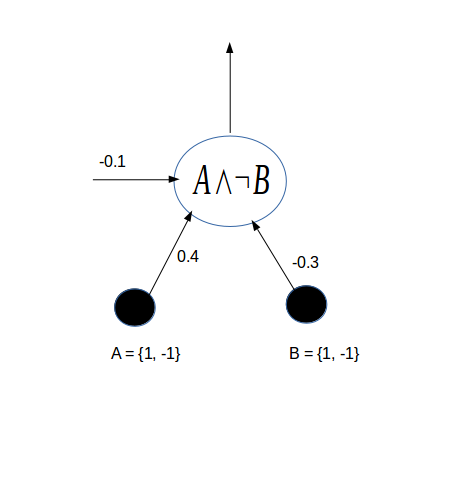
\includegraphics[scale=0.5]{image1}
    \item[b)] Конструирайте мрежа от персептрони, разположени на 2 нива, имплементираща
булевата функция $A \oplus B$

\paragraph{Решение:}\mbox{}\\\\
$$A \oplus B = ( A \land \neg B ) \lor ( \neg A \land B )$$
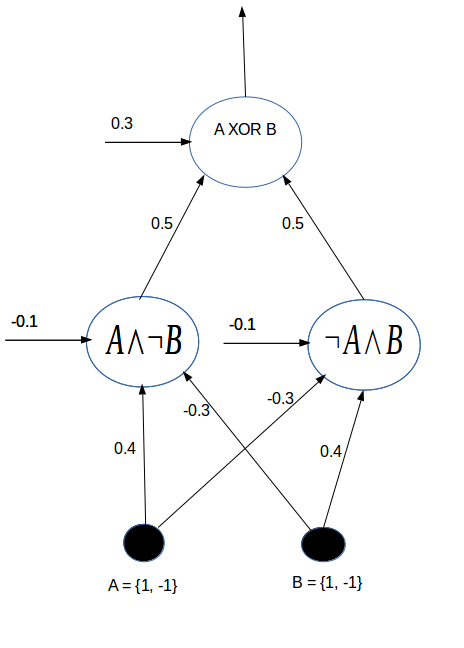
\includegraphics[scale=0.5]{image2}
\end{enumerate}

\paragraph{3)} Изведете правилото за обучение чрез градиентното спускане на един линеен
възел, чийто изход $o$ се задава от формулата:
$$o = w_0 + w_1 \cdot x_1 + w_1 \cdot x_1^2 + ... + w_n \cdot x_n + w_n \cdot x_n^2$$

\paragraph{Решение:}\mbox{}\\\\
Имаме следната функция на грешката:
$$E(\overrightarrow{w}) = \frac{1}{2} \sum_{d \in D} (t_d - o_d)^2$$
където $D$ е множеството от обучаващи примери, $t_d$ е целевият изход, а $o_d$ е
изходът на линейния възел за обучаващия пример $d$.\\
Сега да изчислим градиента на $E$ по вектора $\overrightarrow{w}$:
$$\triangledown E(\overrightarrow{w}) = 
\left[ 
	\triangledown E(w_0), \triangledown E(w_1), \cdots, \triangledown E(w_n)
\right]$$
където:
$$\triangledown E(w_i) = \frac{\partial E}{\partial w_i}$$
$$w_i = w_i - \eta \cdot \frac{\partial E}{\partial w_i}$$
\begin{multline}
\frac{\partial E}{\partial w_i} = \frac{\partial}{\partial w_i} \frac{1}{2} \sum_{d \in D} (t_d - o_d)^2 = \\ = \frac{1}{2} \sum_{d \in D} \frac{\partial}{\partial w_i} (t_d - o_d)^2 = \frac{1}{2} \sum_{d \in D} 2 \cdot (t_d - o_d) \cdot \frac{\partial}{\partial w_i} (t_d - o_d) = \\ = \sum_{d \in D} (t_d - o_d) \cdot \frac{\partial}{\partial w_i} (-o_d) = \sum_{d \in D} (t_d - o_d) \cdot \frac{\partial}{\partial w_i} (-w_0 - w_1 \cdot x_1 - w_1 \cdot x_1^2 - \cdots - w_n \cdot x_n - w_n \cdot x_n^2) = \\ =  \sum_{d \in D} (t_d - o_d) \cdot (-x_i - x_i^2)
\end{multline}
$$w_i = w_i - \eta \cdot \sum_{d \in D} (t_d - o_d) \cdot (-x_i - x_i^2)$$












\end{document}
